\chapter{交互实现及验证实验}

% todo: 介绍第四章完成之后,有了实验平台之后,可以利用实验平台对按照第三章的设计思路探索具体的设计应该如何实现

在第三章我们通过交互研究,发现了大量待解决的交互问题,并得出对应的设计思路有三条:支持可持续使用、系统可解释性、日常可用性。

% 根据设计思路,我们可以通过上一章实现的实验平台逐一进行交互实验。而通过增加系统可变性来支持用户的持续使用,需要大量相关的医学知识的相关数据库,实现起来需要较长的时间和大量的工作量,本章并没有完全实现支持持续使用的所有设计思路,而是只实现了前后结果对比,具体在后续的增加日常可用性的实验中介绍。

% 基于上一章节的工作,接下来的实验工作只需要利用实验平台的提供接口完成客户端原型便可开始实验。


% 本章的实验分别是探索如何增加日常可用性和系统可解释性的实验。 
基于上一章节的工作,接下来我们可以利用实验平台的提供接口快速完成增加日常可用性和系统可解释性原型的开发和实验。
同时,通过这两次实验,也间接验证了实验平台的稳定性和功能可用性。具体的实验内容如下:

\begin{itemize}
	\item 实验1:日常可用性。去掉了强制的操作流程,基于用户更大的自由度的思想,探索了如何实现解决用户日常可用性问题的新设计。

	\item 实验2:系统可解释性。我们通过添加解释来实现系统可解释性,探索了如何增强日常场景下面诊过程中的可解释及其效果,如面诊、舌诊、问诊、结果的解释,影响权重的解释以及通过实验探索添加解释的作用。
	
\end{itemize}

为了能够让用户顺利完成面诊的流程,原型系统需要提供图片预处理的功能帮助用户选取图片和裁剪图片,同时登录注册功能用于在日志中标识用户信息。其中,用户登录和诊断记录查看及图片预处理是各个原型系统通用的功能,健康诊断和健康报告在不同的原型中实现稍微有不同。因此接下来先介绍各个原型系统的通用功能,然后依次单独介绍两个实验。

\section{实验原型通用功能}
通用功能主要包括用户登录、诊断记录和图片裁剪等,采用MUI+AngularJS作为主要开发框架,结合大量插件完成具体实现。客户端通过调用实验平台提供的模型接口,让用户完成诊断的过程。

\begin{figure}[h]
    \centering
    \subfigure[用户登录]{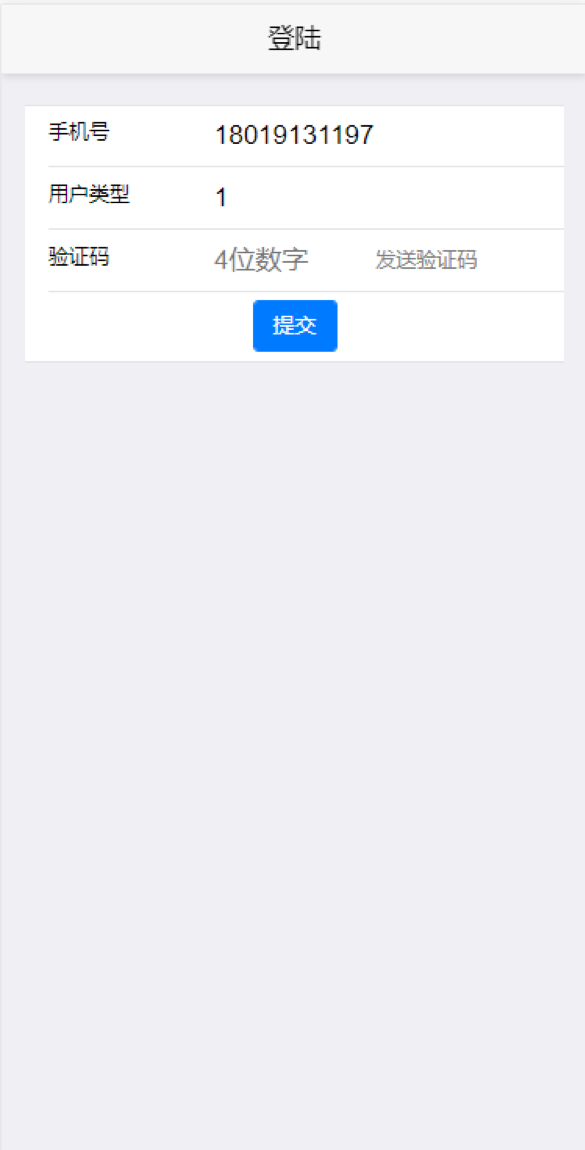
\includegraphics[width=4.5cm]{images/login.png}}
    \subfigure[诊断记录列表]{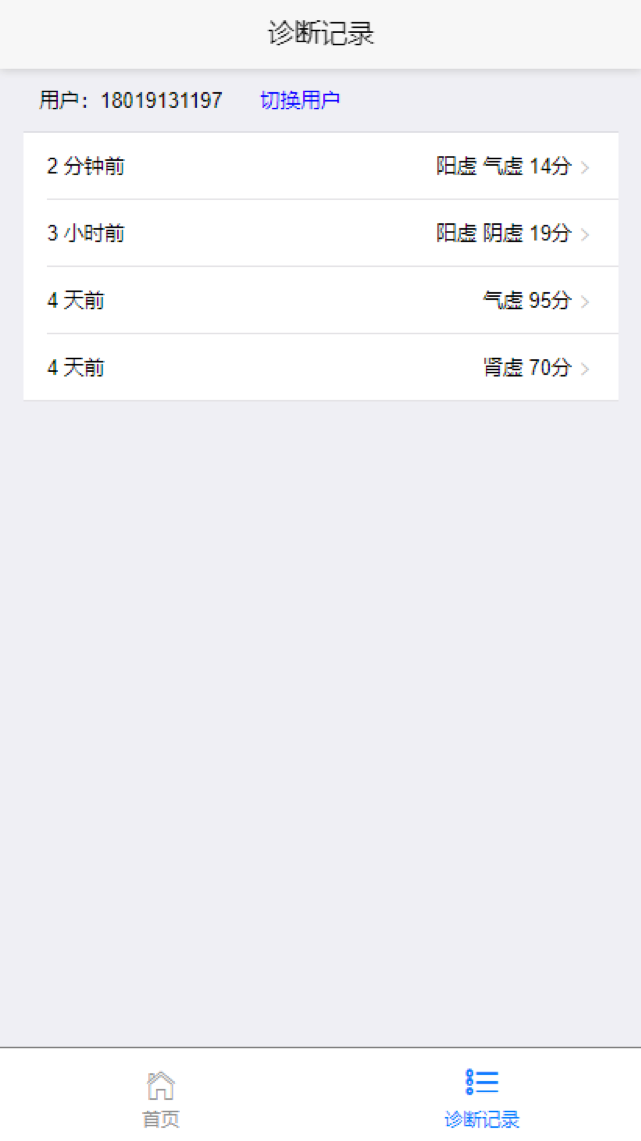
\includegraphics[width=4.5cm]{images/history.png}}
    \subfigure[图片裁剪]{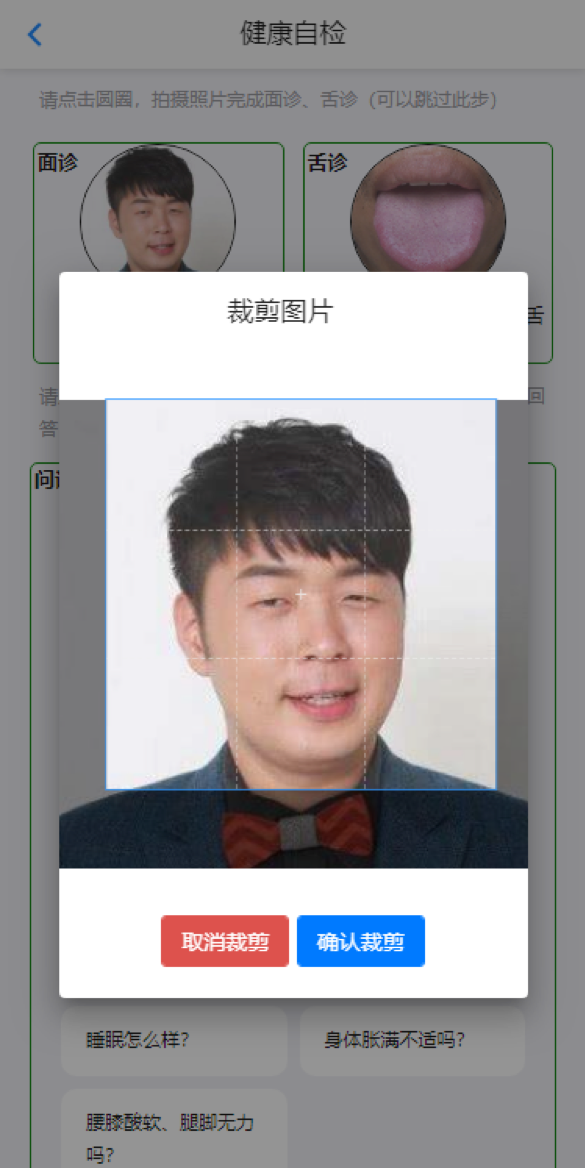
\includegraphics[width=4.5cm]{images/crop.png}}
    \caption{客户端实现}
    \label{fig:client}
\end{figure}

\subsubsection{用户登录}

当用户进入任意页面时,如果发现用户没有登录,会默认跳转到用户登录页面要求用户登录。

如图 \ref{fig:client} (a) 所示,用户登录时,需要输入正确的手机号才能通过手机格式验证发送验证码到手机上。

问了支持第三方问卷系统的跳转登录界面接收一个ssojump参数,用于判断是问卷来源。如果验证通过,则直接跳过登录进入首页。ssojump参数,是问卷星由问卷星平台提供的每一份问卷的唯一标识,是作为实验平台和第三方问卷系统关联的主要依据,因此客户端后续的日志,都需要带上ssojump的参数。

为了支持与第三方问卷系统的数据关联,日志记录时,上传的记录的附加信息为:问卷系统简写字母+问卷系统提供的标识。在本次客户端实现中,采用的是记录标识为wjx-ssojump的方式。

\subsubsection{诊断记录列表}

如图 \ref{fig:client} (b)所示,诊断记录页面,给出用户近期的健康变化的情况。用户可以点击诊断记录,进入当时的详细诊断结果页面。

\subsubsection{图片裁剪}

如图 \ref{fig:client} (c)所示,用户通过点击面诊或者舌诊,可以从相册选择或者通过拍照,上传自己的脸部或者舌头照片。
图片裁剪功能通过调用cropper.js\footnote{https://github.com/fengyuanchen/cropperjs} 实现,用户点击点击确认裁剪后,通过对图片进行base64编码上传到服务器的诊断接口,服务器调用模型池对应模型,拿到子任务结果。

图片裁剪可以帮助用户定位面部和舌头的位置,提高后续诊断的精度。用户点击确认裁剪之后,图片分析结果会直接显示。同时,如果没有识别到人脸或者舌头也会提示用户重新拍照。


\section{实验1:日常可用性设计实现与验证}

% 介绍原设计存在的缺点

% 在之前的研究中我们发现,目前的面诊交互设计在用户日常使用过程中存在以下问题:
在之前的研究中我们发现,目前的面诊交互设计在用户日常使用过程中存在以下具体的可用性问题:
\begin{itemize}
    \item 舌诊、面诊不能可选。与诊所环境不同,由于文化敏感性的问题,大部分中国人认为公共场合伸出舌头是非常不雅观的行为;部分用户也因为各种原因不愿意在非私人空间下拍自己的面部。这种设计对用户的日常使用产生了非常大的阻碍。
    \item 操作繁琐。在用户持续使用的时候,用户每次诊断和上一次通常没有太大的变化。每次让用户重复相同的操作不仅非常费时,而且影响使用的积极性。
\end{itemize}

根据第三章增加日常可用性的思路,本文同样用让用户参与设计过程的设计方法,通过实验平台在线更新设计原型的版本,邀请用户在日常使用的过程中参与迭代过程,最后实现了可用性设计原型。

\subsection{可用性设计原型实现}

\begin{figure}[h]
    \centering
    \subfigure[原型入口]{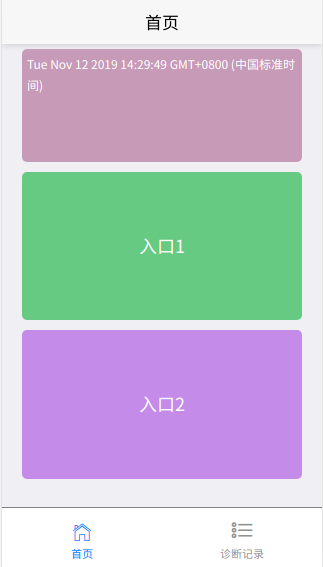
\includegraphics[width=4.5cm]{images/rukou.png}}
    \subfigure[新设计]{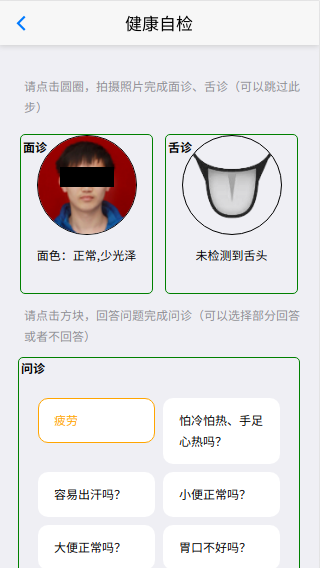
\includegraphics[width=4.5cm]{images/dialog1.png}}
    \subfigure[原设计]{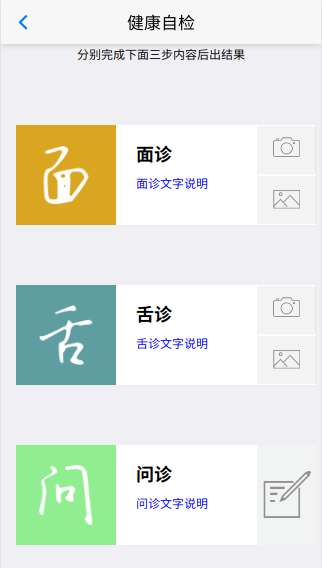
\includegraphics[width=4.5cm]{images/dialog2.png}}
    \caption{日常可用性验证实验}
    \label{fig:interface}
\end{figure}


在原始的云中医的设计中,用户在进行面部舌部拍照后,没有任何提示。具体的结果需要在用户一次回答13个问题之后,点击诊断才能知道面诊是否成功。
本文在实验平台上,实现了一个用于对比的原型系统, 如图\ref{fig:interface} 所示。在该原型系统的首页,有两个入口,新设计和原设计分别对应本文的设计和云中医的设计,两个设计的功能相同。用户在进入实验原型系统的首页之后,可以自由选择入口,进入对应的界面完成诊断。
新设计和之前版本的云中医界面不同的是,诊断界面不仅提供了面诊舌诊问诊的入口,同时会将面诊舌诊的照片和中间结果直接显示在当前页面,用户能对于自己当前身体情况一个直观的感受。

\subsubsection{迭代过程}
\begin{figure}[h]
    \centering
    \subfigure[设计1]{
        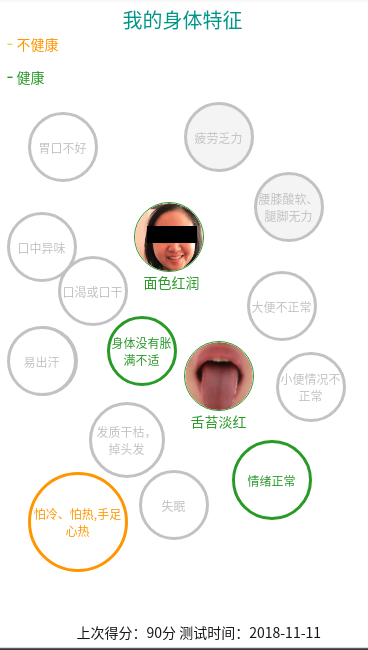
\includegraphics[width=3.5cm]{images/old1.png}
    }
    \subfigure[设计2]{
        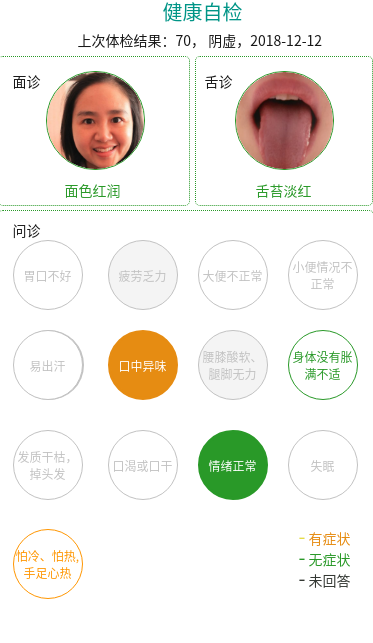
\includegraphics[width=3.5cm]{images/old2.png}
    }
    \subfigure[最终设计]{
        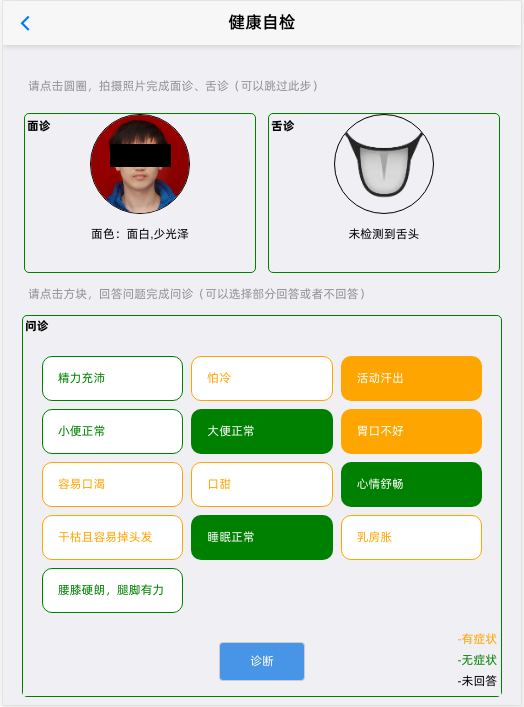
\includegraphics[width=4.5cm]{images/ui-1-1.png}
    }
    \caption{新设计迭代过程}
    \label{fig:diag_new}
\end{figure}
在进行可用性设计的过程中,原型系统经历了多次迭代。每次完成一版之后,我们会邀请小部分用户进行试用收集反馈并及时修改。
图\ref{fig:diag_new} 展示了部分中间的迭代版本和最终设计,其中设计1中的圆圈代表用户需要回答的问题,圆圈的大小代表影响的权重;
设计2简化了界面,统一了圆圈的大小;
最终设计进一步简化了界面元素,并把圆圈改为长方形,方便显示更多的提示信息。

\subsubsection{面诊问诊设计}

\begin{figure}[h]
    \centering
    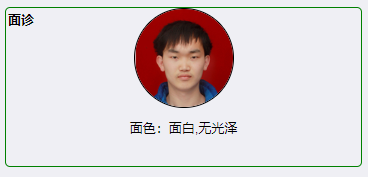
\includegraphics[]{images/diag_design.png}
    \caption{面诊元素设计}
    \label{fig:diag_design}
\end{figure}

根据日常可用性的设计思路,新设计简化了诊断的流程,面诊舌诊问诊在一个页面显示,并且所有的问题和操作都是可选的,不会出现必须要先面诊然后舌诊然后才能问诊的问题。其次,如图\ref{fig:diag_design}所示,新界面对面诊和舌诊进行了中间结果的反馈,面诊在用户拍照确认之后,会立即报告本次照片是否合格已经诊断的结果,用户不需要在点击诊断的时候才被提示照片不合格。

\subsubsection{问诊元素设计}
在问诊方面,新系统实现了最近一次记录保存,由于问题是可选回答的,所以用户只需要回答和自己上次的结果不一致的即可。

\begin{figure}[h]
    \centering
    \subfigure[上次回答有症状]{
        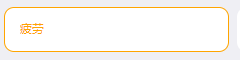
\includegraphics[width=6cm]{images/question/5.png}
    }
    \subfigure[上次回答无症状]{
        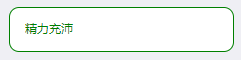
\includegraphics[width=6cm]{images/question/4.png}
    }
    \subfigure[本次回答有症状]{
        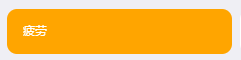
\includegraphics[width=6cm]{images/question/2.png}
    }
    \subfigure[本次回答无症状]{
        
\includegraphics[width=6cm]{images/question/3.png}
    }
    \subfigure[未回答]{
        
\includegraphics[width=6cm]{images/question/1.png}
    }
    \caption{问诊元素的状态}
    \label{fig:question_status}
\end{figure}

同时,如图\ref{fig:question_status}所示,我们对不同问题的回答结果进行了颜色的区分。有色实心代表本次回答,有色空心代表上次回答;橙色代表有症状,绿色代表回答的问题表现良好,没有症状;白色没有填充和边框,为黑字,代表未回答。实心颜色的代表的是用户本次有修改的问诊部分。

在方框内部的问题描述设计上,我们把默认的文字描述,显示为问题描述;一旦用户本次或者上次回答过该问题,则直接显示用户回答的结果。这样做的结果是,第二次用户点进来,就能看到上次的回答结果,这样能够对自己的身体情况有个快速的了解。


\subsection{实验设计}
为了验证本文设计的交互界面的有效性,本文设计了一个交互验证实验,用于验证客户端的实现是否解决了交互的可用性问题。实验流程如下:
\begin{enumerate}


    \item 通过海报(如图 \ref{fig:poster}所示,具体内容有对应的修改)和社交媒体,招募到了12位对中医感兴趣的志愿者参与了本次实验。

    \item 在招募到志愿者之后,我们通过实验平台的问卷关联功能,让每个用户填写一个志愿者的基本信息的问卷,然后单独给每位志愿者介绍我们这次实验的背景和这次实验的整个流程。

    \item 通知用户回家自由使用,我们可以通过实验平台的用户操作记录管理功能观察用户的使用日志,实验期间用户也可以随时反馈使用感受。

    \item 用户持续使用了大概两周之后,单独对每位用户进行深度访谈,通过录音的方式记录访谈数据。

\end{enumerate}

\subsection{实验结果}


\begin{figure}[ht]
    \centering
    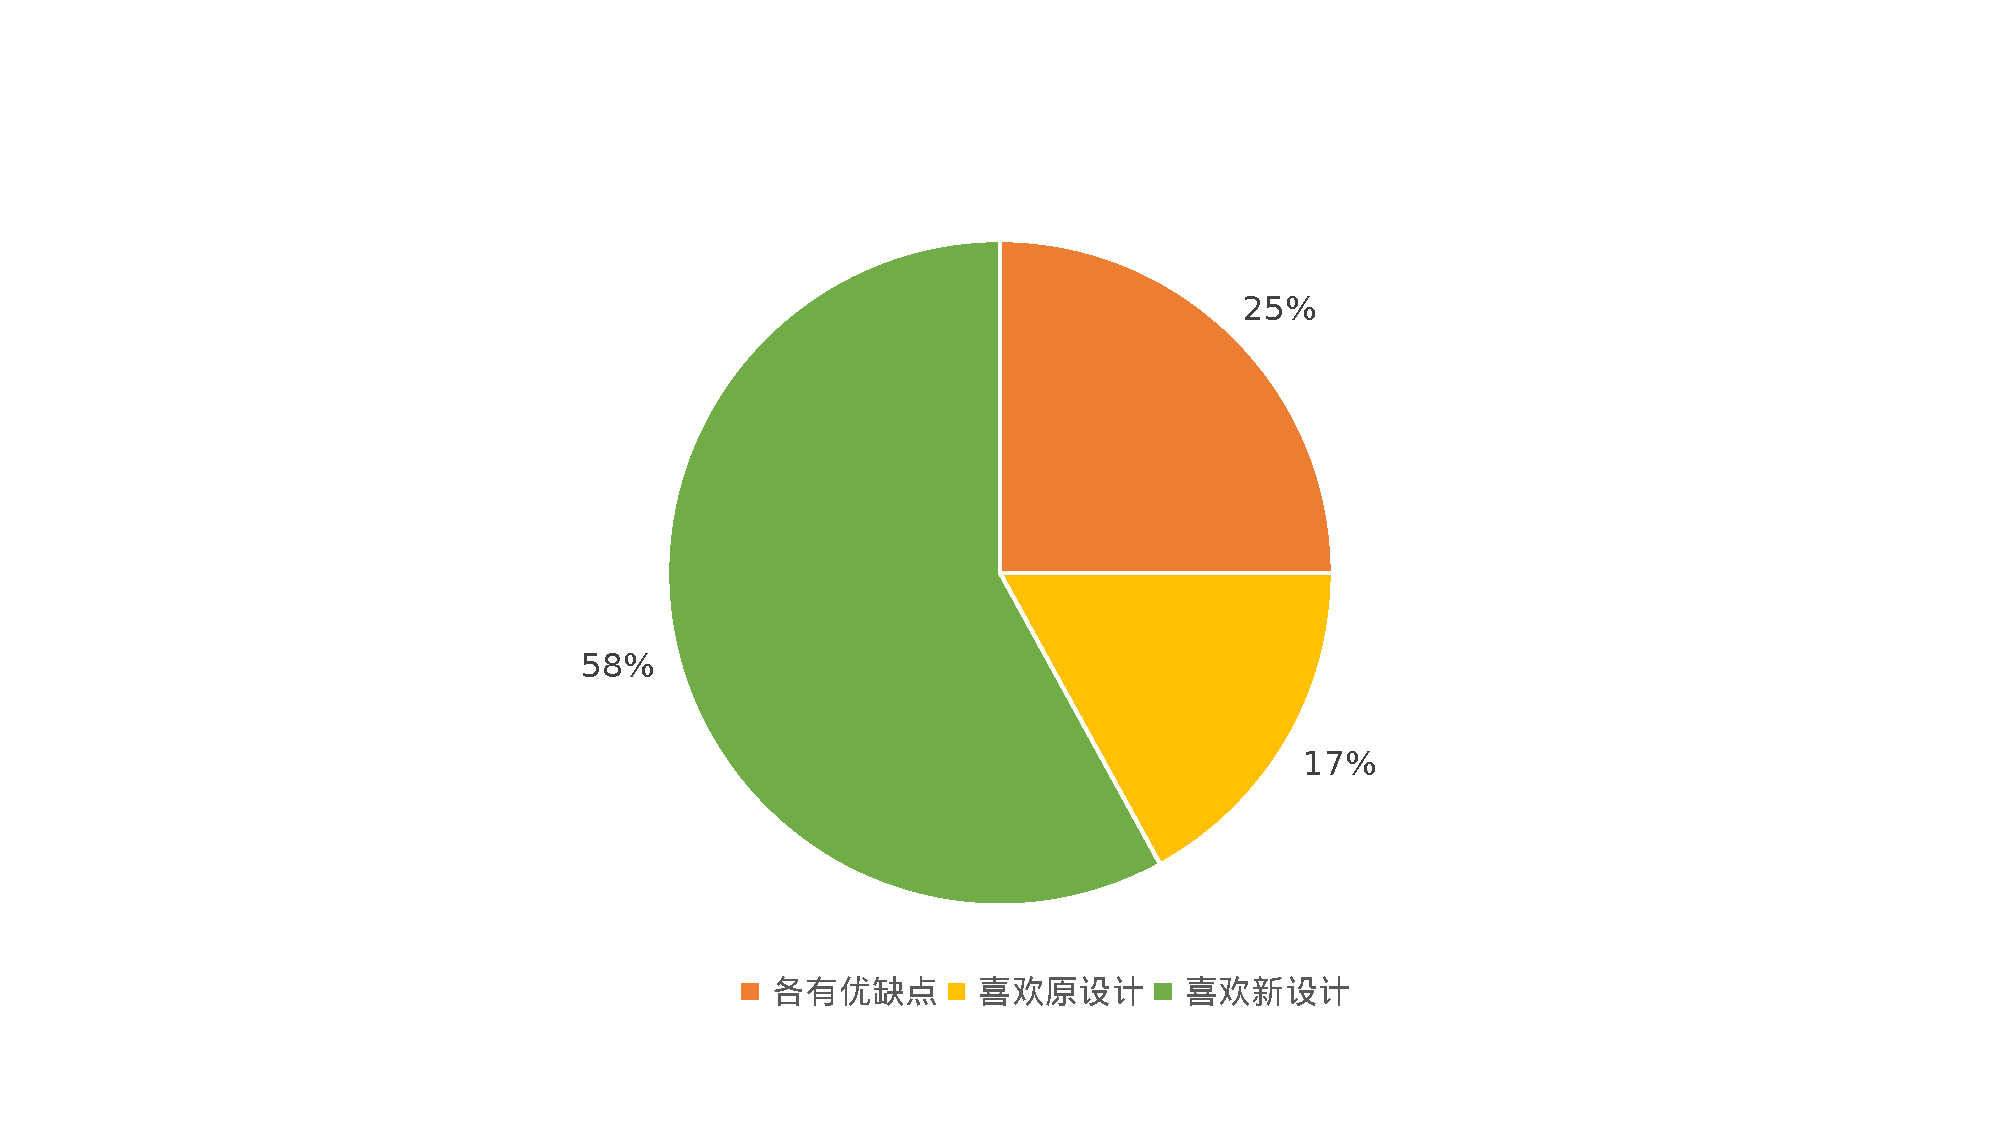
\includegraphics[height=8cm]{images/ui-exp.pdf}
    \caption{界面设计实验结果}
    \label{fig:ui-exp}
\end{figure}

如图 \ref{fig:ui-exp}所示,有少量志愿者选择持续使用原设计完成诊断,大部分用户更喜欢本文的新设计并且原因与用户调研的结果一致,而剩下部分用户觉得两种设计各有优缺点,具体原因如下:


\subsubsection{喜欢新设计}

和之前的用户调研的结果类似,新设计的确能够解决用户的部分日常可用性问题。

根据访谈数据,其中一位参与者认为新设计可以让他在日常使用时只完成自己想做的部分,更加方便:
\myfont{新设计方便,单独做某一块检测;给的指示不空洞;有针对性和选择性。}、\myfont{设计挺好的,感觉更方便一些。}

如我们的预期,新设计带来的可选择性同样在参与者的身上得到了反馈:
\myfont{新设计诊断透彻到位;可以选择性地做诊断,知道健康得分的构成,帮助了解中医知识,省时间。}、
\myfont{新设计操作更简单,有选择性,但是问诊的选项太少,涵盖不全。}

另一部分参与者虽然觉得新设计不好看,但是相对于原先缺乏可用性的设计,新设计基本解决了他的问题:
\myfont{虽然新设计界面丑,但原设计问诊很烦,而且新设计能实时显示舌诊结果。}、\myfont{想按照顺序回答问卷,新设计问诊界面不舒服;但是新设计的选择性检测比较方便。}


\subsubsection{喜欢原设计}
虽然新设计的设计理念是为了方便用户的持续使用,但也同样增加了界面的复杂度。

在选择使用原设计版本的用户中,其中一位参与者就认为新的设计对于他没有帮助而更喜欢一开始有模拟传统中医面诊流程感(先面诊舌诊再问诊)的原设计版本:\myfont{原设计界面好看,问诊流程有完成感,并不想知道具体的症状对应什么细节。}
而另一位参与者则认为问诊应该一次性全部完成,这样在操作上感觉更加连贯:\myfont{原界面设计更符合常规,问诊是连贯的,首页内容很清楚。}

本文提出的设计,虽然能够简化用户的操作,但是会让用户失去自己完成诊断的流程感。
新设计选择了一次性展示用户上次的诊断结果,但是本文的设计在内容丰富度和简单性的取舍下,选择了没有显示原有的问题和所有的选项,用户反馈这种代替用户做选择的方式让用户觉得没有参与感。
当用户希望得到更加准确的面诊结果的时候,繁琐的操作是可以忍受的。

\subsubsection{各有优缺点}
部分用户在实验过程中,两个设计的版本都在交替使用,也难以确定哪一个版本更加喜欢:
\myfont{界面设计更符合常规,问诊是连贯的,首页内容很清楚;新设计圆圈里的不同颜色有提示功能。}、
也有部分参与者反馈新设计并没有符合我们设计的预期,一次性展示所有的选项同样会让用户觉得所有的选项都必须选择:
\myfont{想按照顺序回答问卷,新设计问诊界面不舒服;但是新设计的选择性检测比较方便。}、
\myfont{新设计更方便,但一个一个问题点开很烦;原设计流程顺利,简单。}

\subsubsection{操作耗时对比}

\begin{figure}[ht]
    \centering
    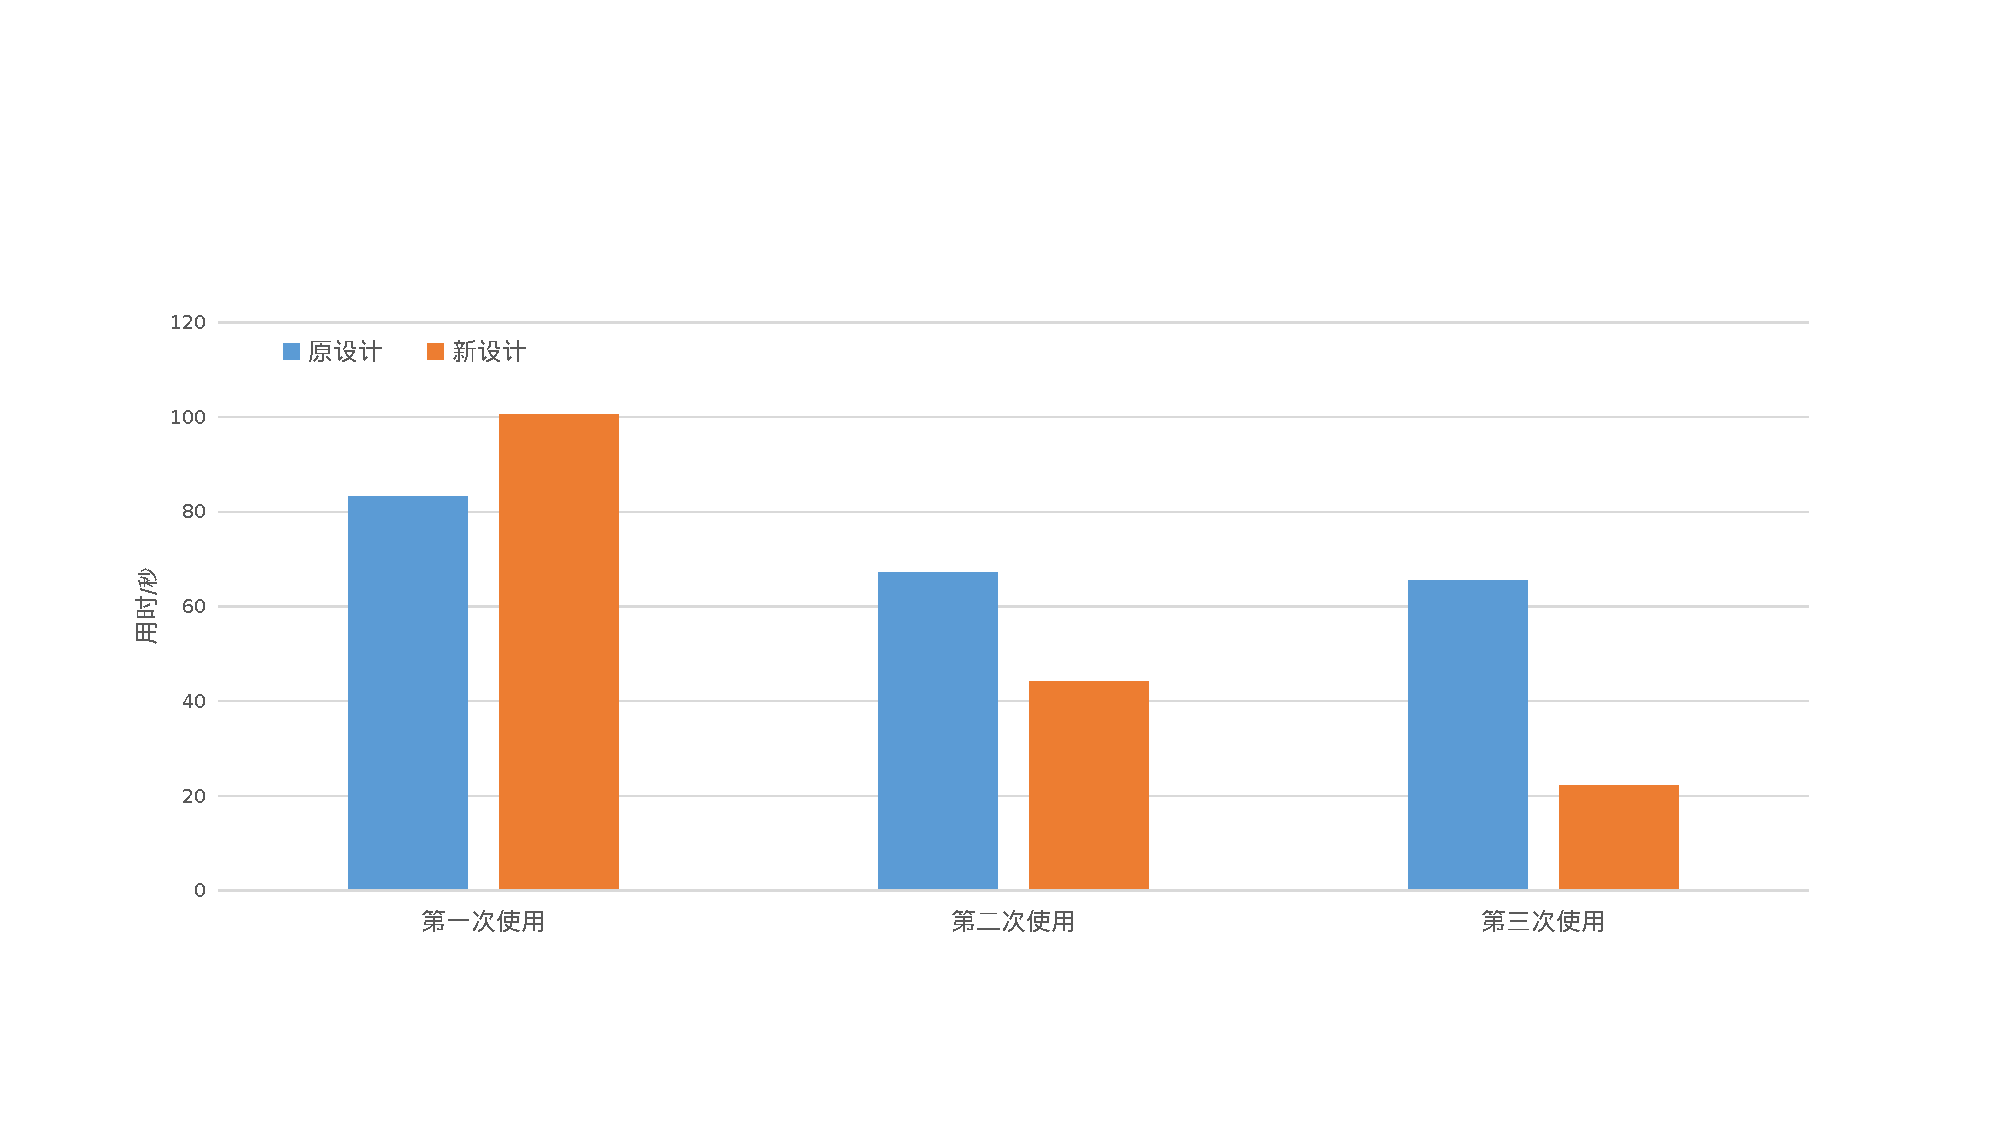
\includegraphics[width=13cm]{images/time.pdf}
    \caption{操作耗时}
    \label{fig:ui-time}
\end{figure}

由于大部分参与者在实验过程中使用系统进行诊断的次数不多,因此本文只通过部分用户的操作日志统计了前三次从进入诊断页面到完成诊断的时间,数据经过处理后的具体结果如\ref{fig:ui-time}所示:

\begin{itemize}

    \item 第一次完成面诊的操作耗时,新设计相比原设计对于用户来说需要更长的时间。如之前的参与者的反馈,新设计没有原设计直观和简单,由于界面相对复杂,因此用户理解后顺利完成诊断需要的时间也比较长。

    \item 在后续的第二次、第三次操作中,旧设计的操作时间在用户熟悉之后稍有降低,但是总体来说变化不大;新设计可以让用户直观的看到自己上次的面诊舌诊数据和问诊的选择,用户可以只选择完成有变化的部分实现快速诊断,完成一次操作时间大大降低。

\end{itemize}

\subsubsection{总结}
通过实验,我们发现新的设计在一定程度上的确解决了本文在之前提到的可用性问题。用户在日常使用的情况下能减少用户在完成诊断操作上花费的时间。
不过值得注意的是也有部分年纪较大的用户反馈新的设计过于复杂。总体来说符合日常可用性设计思路的预期,能够满足用户日常使用的需要。
% 没有依次做完面诊、舌诊、问诊的完成感,没有做到兼顾所有用户的需求。

\section{实验2:系统可解释性设计实现与验证}

% \cite{wang2019designing, lim2009and}

根据之前的用户调研的结果来看,当前系统存在以下问题:

\begin{itemize}
    \item 由于当前诊断和打分模型存在改进的空间,部分的用户对结果产生了怀疑或者对结果不理解的问题。
    \item 日常场景下,没有专业医护人员的帮助,普通用户由于缺乏对应的专业知识,对应用的理解还有很大的提升空间。
\end{itemize}

目前主要对提高用户对系统理解程度的方式一般是通过文字、可交互式元素或者可视化的方法描述来暴露算法置信度、暴露中间结果、提供当前数据和原始数据对比等实现\cite{wang2019designing, kocielnik2019will},其中文字化的描述适合对系统的背景、或者专业名词进行解释;暴露算法的中间结果以及置信度,能激起用户探索算法原理的好奇心以及提高对结果的容忍程度。

在这个理论的基础上,我们希望通过将模型的诊断过程对用户可见,并对结果进行解释,来提高用户的交互体验。
但是面诊系统在日常生活中的应用是一个全新的场景,需要解释的对象是什么,通过何种交互元素进行解释,仍是未知的问题。

% 系统可解释性可以通过解释算法置信度、算法中间过程等方式实现。因此我们在尝试系统中加入算法的解释性,提升用户的体验。

% 在这个基础上,我们希望通过将模型的诊断过程对用户可见,并对结果进行解释,来提高用户的交互体验。

% 虽然目前已有相关的对系统进行解释的方法\cite{wang2019designing, lim2009and},如通过解释算法的可信度,暴露原始数据和中间结果,以及通过图表等方式实现结果对比等,增加系统可解释性,可以提高用户的交互体验。

\subsection{可解释设计原型实现}

在第四章中本文详细介绍了目前技术探针中可用的模型,根据本文系统和模型的特点,解释在呈现的时候,实现的解释方法大致可以分为以下几种:

\begin{enumerate}
%  为什么要解释,文字解释的作用。
    \item 如图\ref{fig:face_diags}所示,结果中文字结果有提示、可以进行点击。如果用户点击了健康报告的分数,会通过弹窗通过文字描述进行详细的解释。

    \item 如图\ref{fig:question_weight}所示,通过雷达图的可视化方式直接显示对结果的影响,交互性比较强。 
    
    \item 如图\ref{fig:report_expalin_score}所示,通过可交互元素折叠列表对不同条件下的计算公式进行解释。
\end{enumerate}

用户在使用系统的过程中,需要经过面诊、舌诊、问诊等流程,最终得到诊断的结果。为此我们根据交互研究中用户反馈的问题,对用户完成一次诊断的中间流程以及最终的结果都进行了解释。

\subsubsection{面诊舌诊的解释}

\begin{figure}[htbp]   
    \centering
    \subfigure[不解释]{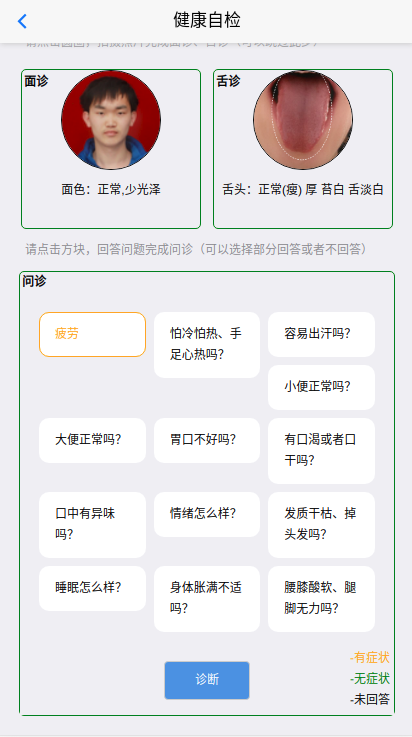
\includegraphics[width=4.5cm]{images/face_tongue.png}}
    \subfigure[解释]{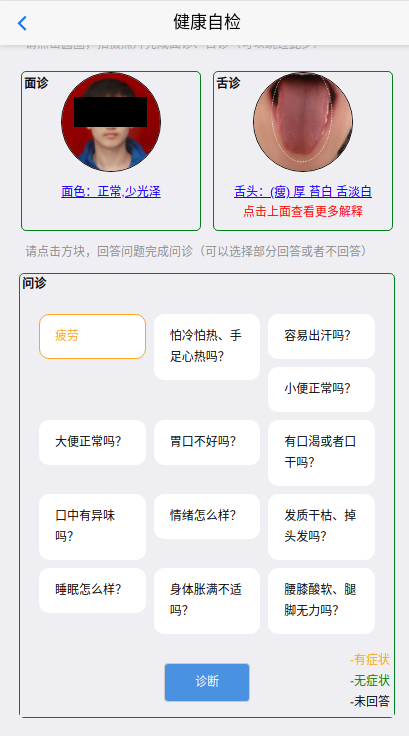
\includegraphics[width=4.5cm]{images/exp_face_tongue.png}}
    \subfigure[详细解释]{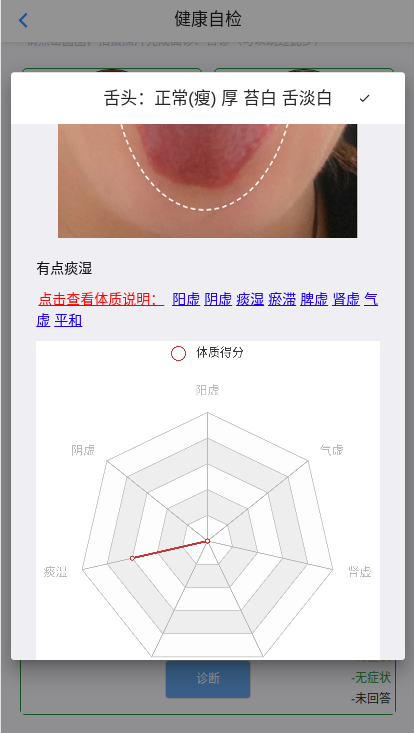
\includegraphics[width=4.5cm]{images/exp_tongue.png}}
    \caption{面诊舌诊的解释}
    \label{fig:face_diags}
\end{figure}

面诊和舌诊流程比较类似,都是通过分析面部或者舌部图片,得到分析结果,因此这两部分合并放到一起解释。
面诊和舌诊断添加解释主要体现在结果的解释,包括中间结果和对各种体质倾向的影响。
用户查看解释之后,能够大致了解本次拍照是否成功,并且知道目前面诊的结果,以及可能会对最终的健康报告造成哪些影响。具体如图 \ref{fig:face_diags} 所示:

(a) 没有解释的设计,只能看到结果。

(b) 有解释的设计,通过点击面诊或者舌诊结果,查看对结果的解释。

(c) 点开解释之后,系统会弹窗进行详细的解释,不仅可以看到当面诊断的中间结果,也能看到这次诊断的体质倾向得分。

接下来介绍该原型中各个解释的细节具体如何实现。


\subsubsection{问诊的解释}

\begin{figure}[htbp]
    \centering
    \subfigure[不解释]{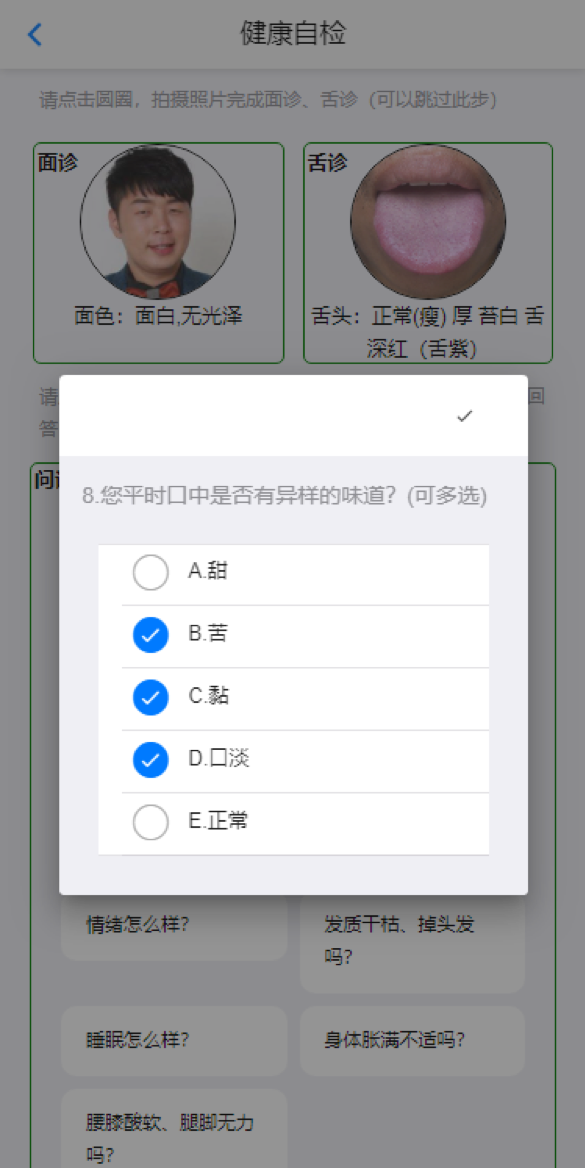
\includegraphics[width=5cm]{images/questions.png}}
    \subfigure[解释体质术语]{
        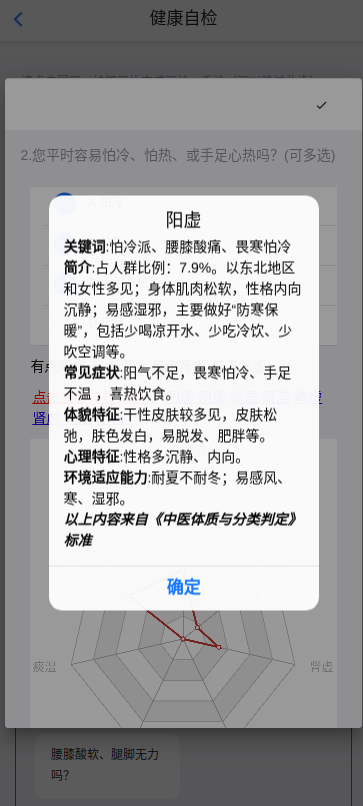
\includegraphics[width=5cm]{images/exp_phy.png}
    }
    \caption{问诊的解释}
    \label{fig:questions}
\end{figure}

问诊的过程中解释的主要实现,是通过对体质的专业术语和每个答案对结果的影响进行解释,具体实现如图 \ref{fig:questions} 所示:

(a) 不解释的设计,用户回答问诊问题之后,没有任何提示或者解释。

(b) 有解释的设计,用户在进行问诊过程中,可以立即看到每个答案对结果的影响,通过下方的雷达图显示了影响的体质倾向类型和具体的数值。
雷达图的更新是实时根据用户的选择进行更新的,用户可以通过点击不同的选项查看不同选项对应的雷达图。

(c) 点开体质的解释之后,会通过弹框的方式,对中医术语中,各种体质的解释。对于体质内容的解释文字引用自 《中医体质分类研究》标准\cite{王琦20099}。


\subsubsection{诊断结果的解释}
\begin{figure}[htbp]
    \centering
    \subfigure[不解释]{
        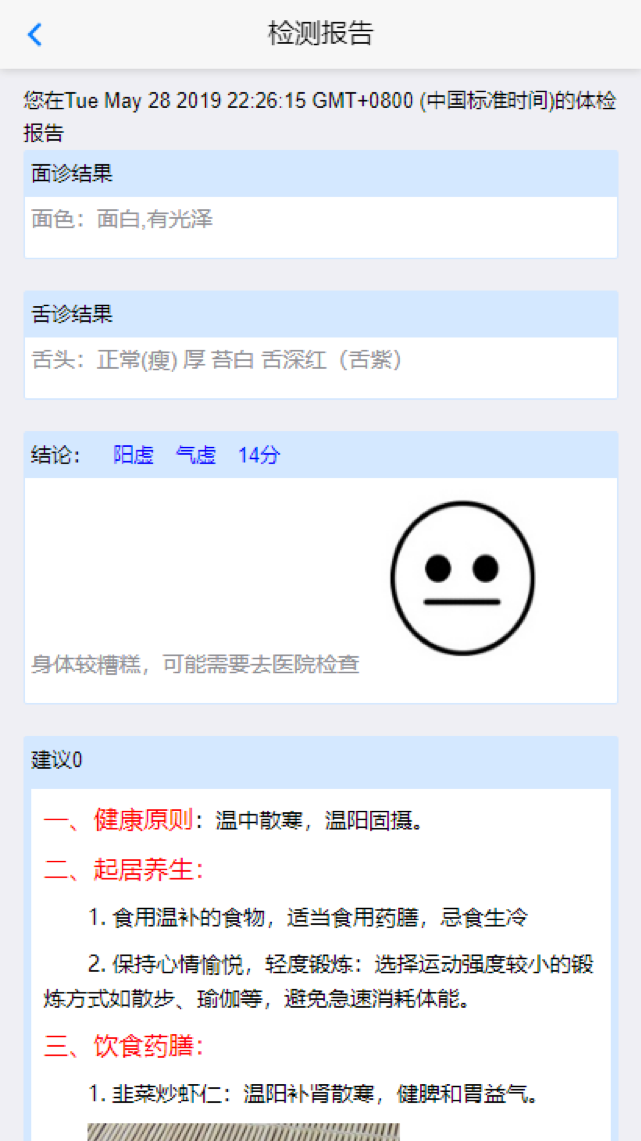
\includegraphics[width=4.5cm]{images/report.png}
    }
    \subfigure[解释]{
        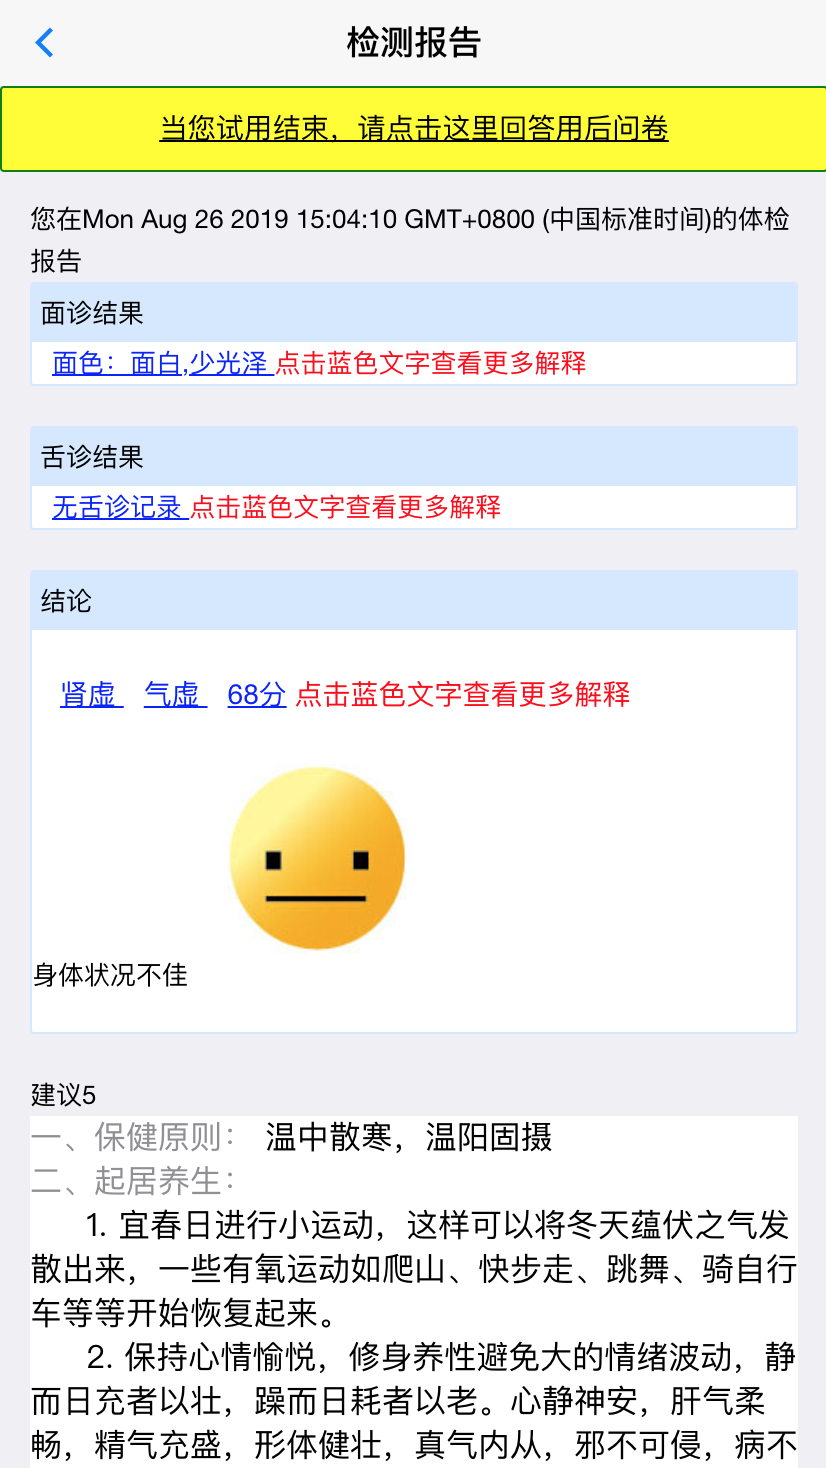
\includegraphics[width=4.5cm]{images/report3.png}
    }
    \caption{诊断结果的解释}
    \label{fig:exp_result}
\end{figure}

诊断结果的解释主要是对结果的判断依据和相关原理进行解释,具体如 \ref{fig:exp_result} 所示:

(a) 在没有解释的设计中,用户在诊断结果页面,可以看到自己的健康分数和体质结果,并且会在后面给出对应的养生建议和实践,但是给出的结果是不可点击的;

(b) 在有解释的设计中,用户可以点击诊断结果,包括面诊结果、舌诊结果,体质、健康分数。用户点击之后,可以通过之后的弹框,看到详细的解释,如点击健康分数之后,可以了解这个分数是根据哪些指标,通过哪一个算法计算过来的。

从\ref{fig:exp_result} 中我们可以看出有解释的设计中,用户点击结果后,会通过弹框解释结果。可以点击查看的结果的解释有:面诊舌诊结果的解释,健康分数的解释,体质的解释,接下来分别介绍如何实现。



\subsubsection{健康分数的解释}
问诊结果的解释主要是对用户解释诊断结果是如何计算,以及那些问诊的问题对结果有影响,影响程度多少。

\begin{figure}[htbp]
    \centering
    \subfigure[相关问题]{
        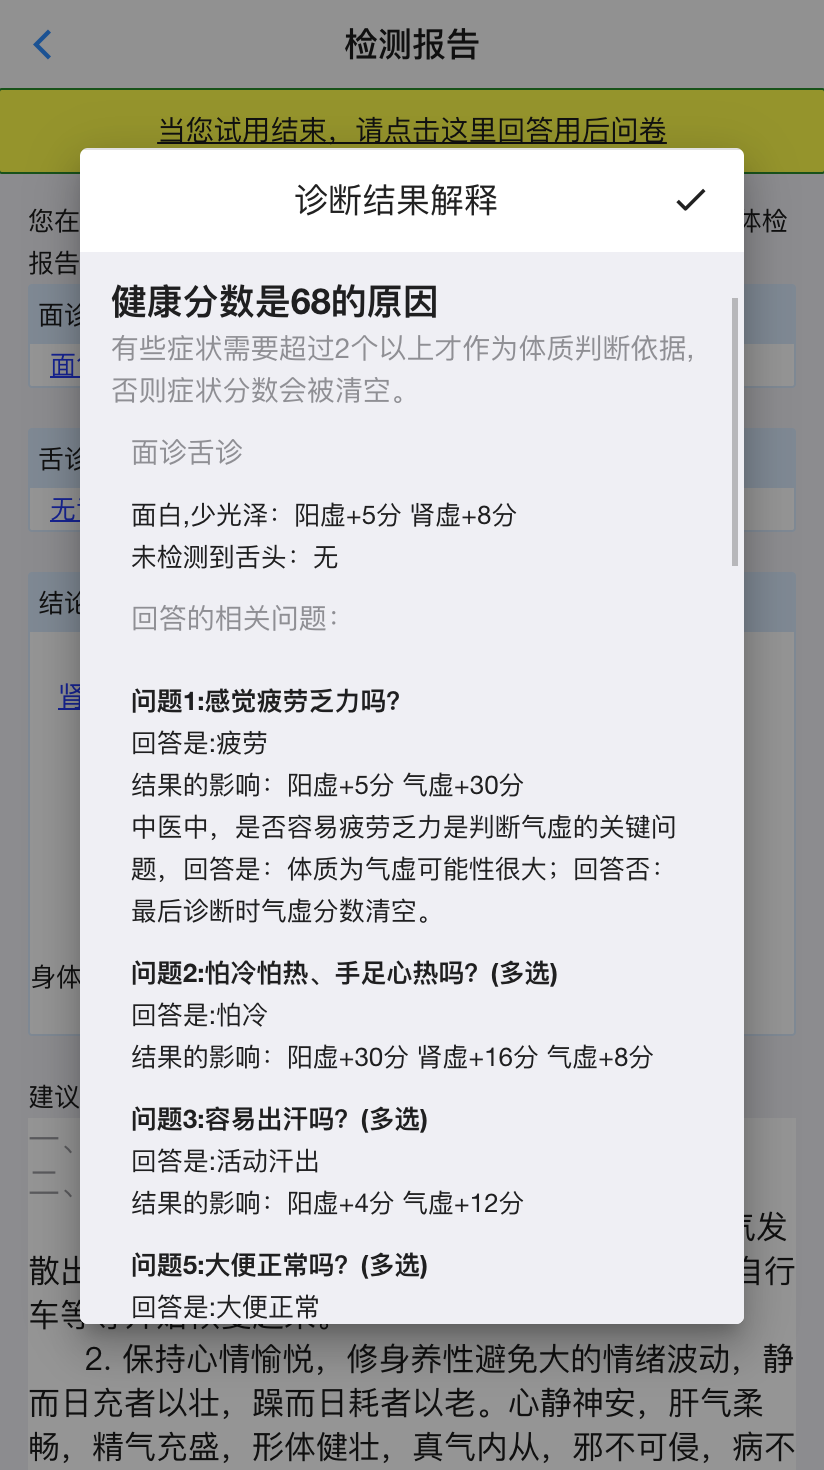
\includegraphics[width=4.5cm]{images/report7.png}
    }
    \subfigure[雷达图]{
        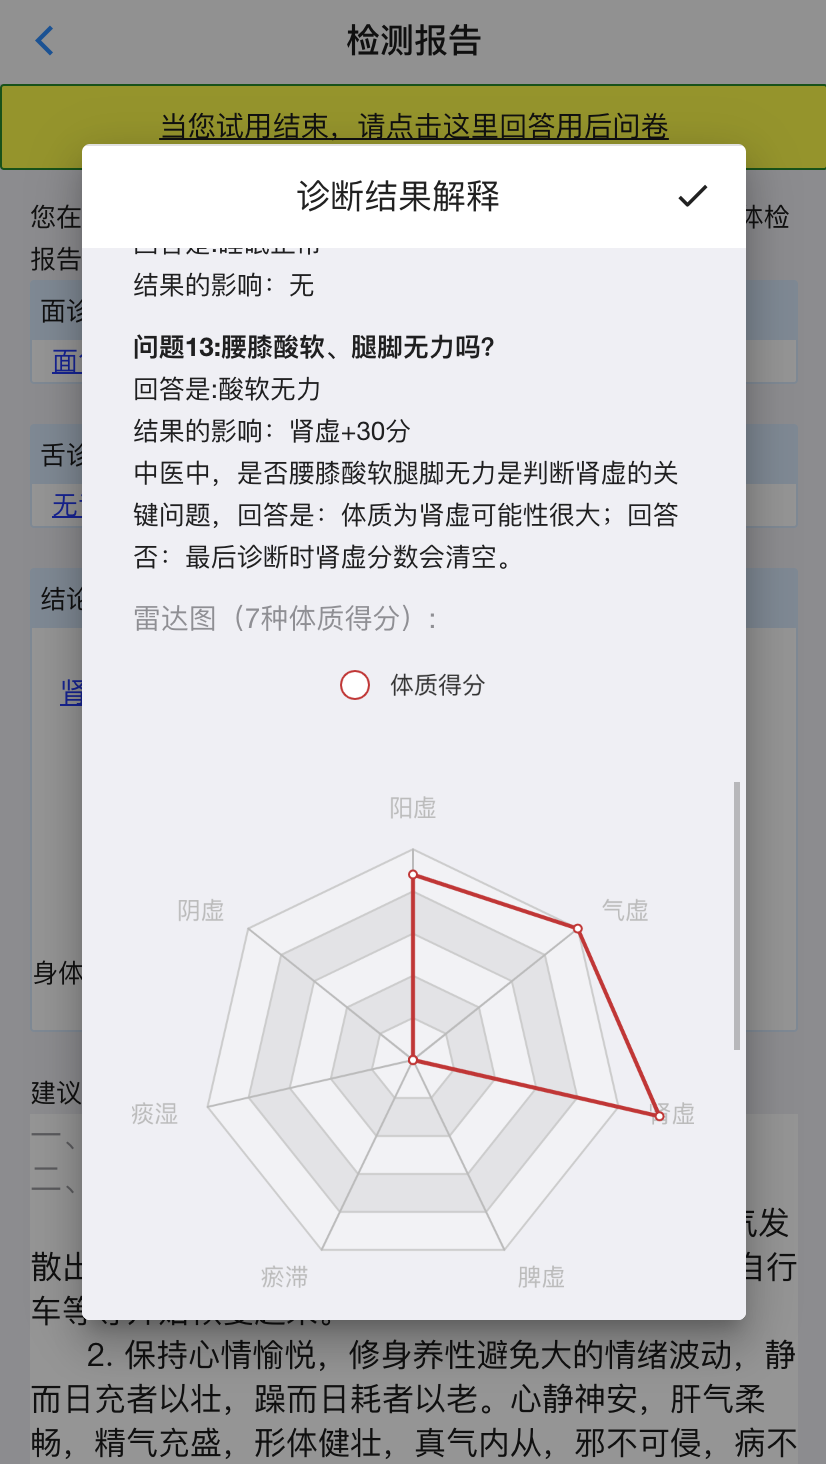
\includegraphics[width=4.5cm]{images/report8.png}
    }
    \subfigure[计算公式]{
        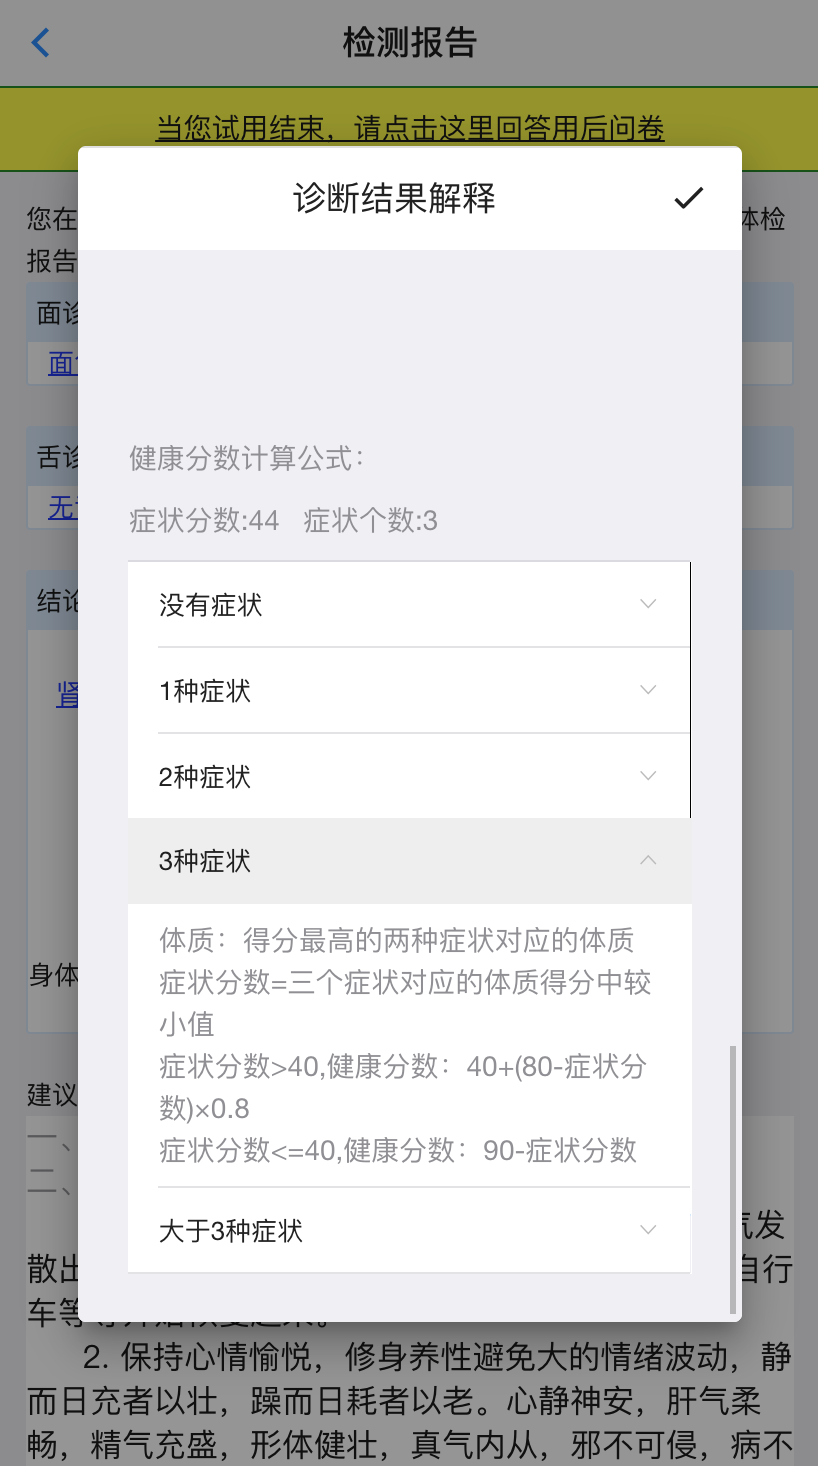
\includegraphics[width=4.5cm]{images/report9.png}
    }
    \caption{健康分数的解释}
    \label{fig:report_expalin_score}
\end{figure}

如图\ref{fig:report_expalin_score}所示,用户点击诊断页面的分数之后,弹窗里会显示分数相关的问题、雷达图和分数计算公式。

分数相关问题,展示了面诊舌诊对体质分数的影响和问诊对体质分数的影响,无影响的问题则不会显示。

用户每次回答一个问诊的问题,或者进行面诊舌诊断,都会对体质的倾向分数产生一定的影响。在规则系统中,体质倾向分数的变化分两种,一个是分数的累加,另一种是体质倾向分数的清空。

雷达图对体质分数进行了汇总,给用户展示最终个人的体质倾向的结果。

根据规则系统,解释页面的计算公式一共有5种类别。用户具体属于哪个类别,使用哪一套计算公式,是由用户当前的症状的个数来决定的。

我们使用选项卡的方式,将所有的打分计算公式全部暴露给用户,并且默认打开当前计算公式的选项卡。

\subsubsection{体质的解释}

\begin{figure}[htbp]
    \centering
    \subfigure[概念的解释]{
        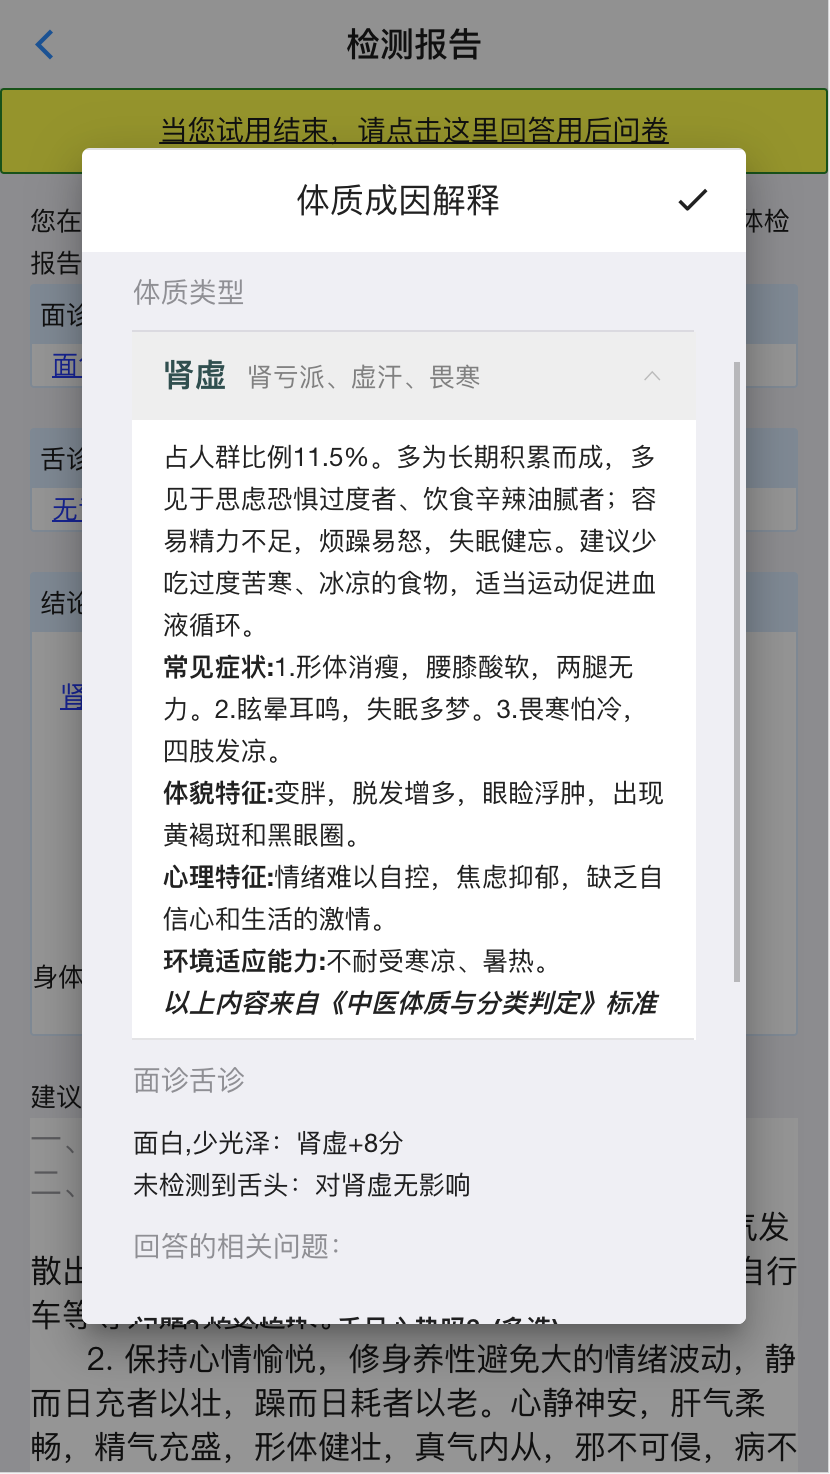
\includegraphics[width=4.5cm]{images/report5.png}
    }
    \subfigure[影响结果相关问题]{
        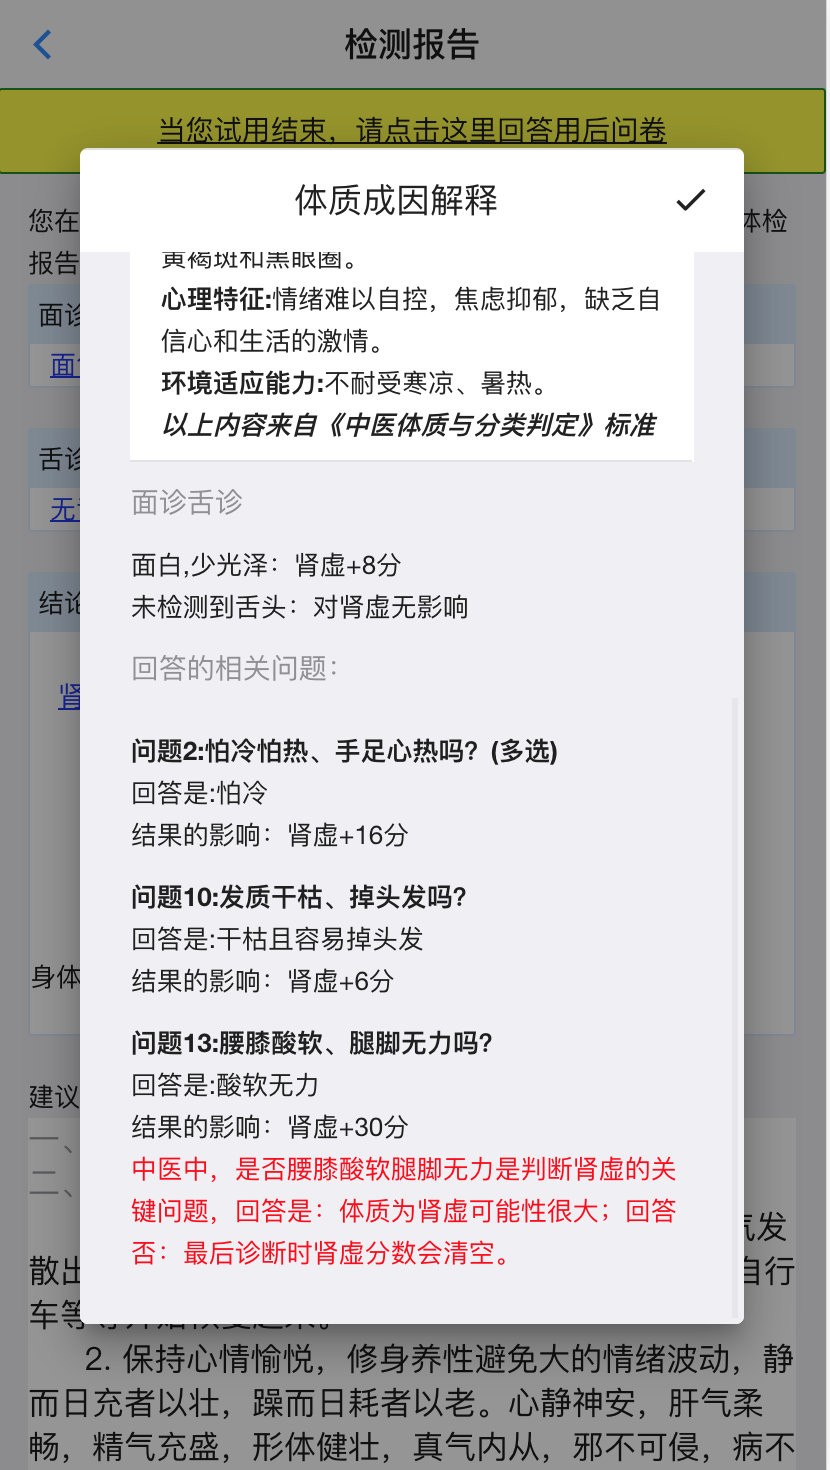
\includegraphics[width=4.5cm]{images/report6.png}
    }
    \caption{体质的解释}
    \label{fig:report_explain_phy_1}
\end{figure}

如图 \ref{fig:report_explain_phy_1} 所示:

(a) 在解释体质结果之前,我们首先对该体质的特征进行了说明,对体质的概念进行了解释。

(b) 后续,我们将规则系统判断时用到的相关的问题暴露给了用户。用户可以看到自己舌诊、面诊或者问诊中回答的某一个问题,对于该结果的影响。
% \section{反馈调研}
% 在新系统完成之后,我们采访了16名用户。
% 在本次调研过程中,用户试用的是同时有新旧界面的版本,除了第一次介绍使用的时候,我们会让用户两个版本都是使用一下,后续不做限时。用户具体使用的时候可以根据自己的喜好选择。
% 经过回访,新设计的界面达到了预期,大部分用户觉得使用起来更加地方便。
% 不过值得注意的是,也有少部分的用户喜欢原设计的将面诊,舌诊,问诊分开为三步进行的方式,因为这样比较符合日常生活的习惯。


\subsection{实验设计}

为了研究如何对面诊系统进行解释,我们设计了一个交互实现,通过线上实验结合深度访谈的形式进行。

\subsubsection{线上实验}
通过在各大社交平台发布海报,以及使用问卷星的样本服务招募志愿者, 经过筛选之后,我们一共招募了60位左右的用户。

每个用户的实验流程如下:

(1)用户通过扫描二维码,或者通过我们给定的链接,进入问卷星的调查问卷。

(2) 完成调查问卷之后,跳转到原型系统。通过调用问卷星提供的企业用户接口, 同时把问卷星的问卷id通过ssojump传给云中医在线应用。
通过ssojump中的问卷id, 完成自动登陆, 登陆的用户id为wjx-{问卷星id}。

(3) 在用户完成一次面诊之后,会在健康诊断页面下,看到一个跳转链接,可以选择填写用后问卷。

在实验过程中,用户会被随机分配到有解释的原型系统和无解释的原型系统。

\subsubsection{深度访谈}

定量的数据分析,我们无法得出哪些因变量如对结果的信任与是否有解释的相关性。于是我们在该次实验之后,对实验的参与者附加了一个深度访谈。

本次实验,我们同样实现了一个原型系统,界面和流程与上一个实验完全相同,但是去掉了用户登录时的随机分配用户角色,而是添加了一个开关。
当开关关闭的时候,系统不会对结果进行解释;当开关打开的时候,系统会对诊断过程和诊断结果进行详细的解释。

在使用过程中,我们首先让用户试用有解释或者没有解释的版本,让用户随时讨论自己内心的想法。然后我们切换开关,让用户再一次使用。最后对用户进行一次深度访谈。

\subsection{实验数据}
每个用户在参与实验之后,我们可以得到调查问卷的数据,云中医的使用日志,已经用后问卷的数据。

\subsubsection{可用数据}
本次实验可分析的数据来自调查问卷,用后问卷和实验平台的日志三个数据表,对应的可用数据如下:

调查问卷:序号,提交答卷时间,所用时间,来源,来源详情,IP,个人信息,我相信中医养生,了解中医养生,平时注重养生,经常去看中医,希望自己的生活方式更健康,对学习相关中医养生知识感兴趣,认为中医面诊可以了解健康情况,认为中医舌诊可以了解健康情况,认为智能系统可以自动评估健康情况,随机顺序的中医知识问题。
其中个人信息包括性别,年龄段,受教育水平,职业,城市,健康状态等。

用后问卷:序号,提交答卷时间,所用时间,来源,来源详情,IP,云中医的诊断结果,结果的信任程度,对结果的理解程度,是否愿意使用类似应用,随机顺序的中医知识问题。

用户使用日志: 序号,用户名,设备信息,操作名,操作信息,日期 。

\subsubsection{信息提取}
对于同一个用户在一次实验过程中,若调查问卷的ssojump参数为ID, 则此次用户操作记录的用户名为wjx-ID, 用户问卷的来源详情为wjx-ID。 
通过这个对应关系,我们就可以利用实验平台提供的问卷关联的功能,把三个表的信息,合并到一个表中,实验平台通过表格插件导出下载,最终得到特征如表\ref{tab:exp_data}所示。


\begin{table}[h]
    \centering
    \begin{tabular}{ll}
        \toprule
        字段 & 描述 \\ 
        \midrule
        序号 & 调查问卷序号 \\
        性别 & 男/女/未知 \\
        教育程度 & 本科以下/本科/本科以上 \\
        工作类型 & 计算机相关/计算机不相关 \\
        用户类型 & 解释/不解释 \\
        健康得分 & 云中医应用给出的分数 0-100 \\
        信任 & 对结果的信任程度 1-5 \\
        理解 & 对结果的理解程度 1-5 \\
        前健康知识得分 & 使用云中医之前的健康知识得分 \\
        后健康知识得分 & 使用云中医之后的健康知识得分 \\
        查看了哪些解释 & 使用过程中查看的解释类型 \\
        \bottomrule
    \end{tabular}
    \caption{实验数据汇总}
    \label{tab:exp_data}
\end{table}

经过处理之后,我们最终得到的数据图表 \ref{tab:exp_data}所示,对应的字段说明如下:

\begin{itemize}
  \item 工作类型: 根据调查问卷的数据,用户自由填写的职业类型有很多,为了便于分析,我们把 IT经理,IT软件设计, hr, it, 互联网, 技术研发, 技术研发人员, 技术经理, 电脑工程师, 研发, 科研, 程序员, 计算机, 软件工程师, 软件开发工程师, 通信, 通讯等归为it相关。

  \item  信任、理解: 这两个字段来自用后问卷调查表,取值范围为1-5的整数。

  \item  健康知识得分: 使用云中医应用前后的健康知识得分,使用的是用户回答正确中医知识的个数。

  \item  用户类型:用户使用的版本,包括原始版本或者添加了解释的版本。

  \item  查看了哪些解释: 通过检索日志中关键字获取,包括面诊过程,舌诊过程,体质术语介绍,诊断报告的:面诊结果,舌诊结果,健康分数,体质,分数计算公式等。
\end{itemize}

\subsection{实验结果}

\subsubsection{影响权重的解释方式}
在面诊舌诊和问诊中,都会涉及到本项的诊断对最终体质影响的权重。我们通过实验发现相对于柱状图的方式,雷达图更加适合该场景。

在权重解释这部分,用户不仅可以看到自己目前的舌相或者面相对应的特征,还能看到对每个体质影响的权重,该原型将最后诊断的规则系统部分规则暴露给了用户。
向用户解释这个权重的时候,我们使用了图表的方式向用户解释权重。如图 \ref{fig:question_weight} 所示,实验迭代的过程中我们先后实现了使用柱状图和雷达图的方式来展示权重。

\begin{figure}[htbp]
    \centering
    \subfigure[柱状图方式]{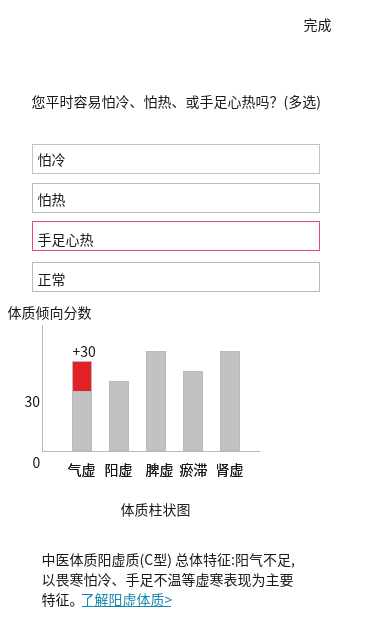
\includegraphics[height=10cm]{images/old3.png}}
    \subfigure[雷达图方式]{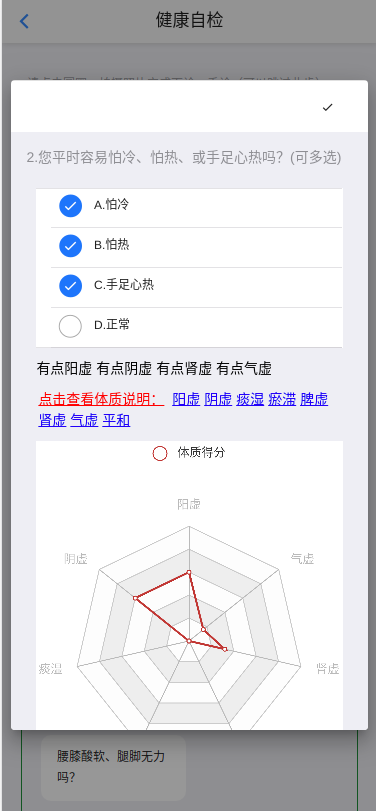
\includegraphics[height=10cm]{images/questions2.png}}
    \caption{影响权重的解释}
    \label{fig:question_weight}
\end{figure}

如图\ref{fig:question_weight}(a)所示,我们在设计中采用柱状图的方式向用户解释该问题对体质倾向影响的权重,其中通过红色突出显示本次出现变化的部分。
但是在实验过程中,经过用户反馈,我们发现在和用户自己健康相关的场景下,柱状图不适合用来解释影响权重。柱状图在权重差距较大的情况下可能会有一部分\myfont{突出}的比较高,有一个明显的缺点就是柱状图容易引起用户对自己身体情况的焦虑感。部分用户的反馈如下:
\myfont{然后他那个柱状图是太让人心慌了,那么片面的每道题给你一个那么高的值。}、
\myfont{下面那个柱状图非常吓人的,弹出来很高,让我有一种我的脾脏已经不行了的感觉。}

为了避免在解释影响权重过程中引起用户不必要的恐慌,我们需要一种相对"温和"的方式对影响权重进行解释,于是最终选用了雷达图的方式来解释影响权重。
如图\ref{fig:question_weight}(b)所示,雷达图从外观上来看会让数值的峰值不那么明显。

\subsubsection{日志分析结果}

通过对在线实验数据变量间的相关性分析,结果并没有体现出各个变量和是否看了解释的有强相关性,当前的解释方式对用户吸引力还不够。

根据日志数据,发现本次实验数据中,大多数参与者的完成质量非常差,具体有以下几个特点:

\begin{enumerate}
    \item 虽然我们在线上收集数据的时候,过滤了完成实验用时较短的样本,但是整体的完成实验的时间也是偏短,说明用户在填写问卷的时候没有认真思考。

    \item 日志数据中用户点击了解释的比例不到1/3,点了解释的用户中大部分也只点了面诊、舌诊、体质解释、结果解释中的一种,剩下的大部分用户并没有去点击去查看解释。
\end{enumerate}

% 同时实验分析,我们可以得出,增加解释可以提高用户对应中医知识的理解。

% 和看解释有关, 用 二元逻辑回归

% 把用户进行筛选,看了解释和没有看解释的

% 有解释的,看了没没看的(为什么看了,为什么没看), 

% 相关性分析,用于分析自变量

% 挑选相关性比较低的,放到后续的模型中 , 不加*,是很弱的 0.4-0.6比较强

% 了解中医养生,平时注重养生,了解中医养生
% 相信中医,了解中医

% 有没有看解释和it相关性不高

% 看了解释的影响:
% 独立样本t检验,差异性分析,没有显著差异

% 找最相似的不看解释的用户和看了解释的用户对比: 
% 对结果的信任和理解程度,两个样本没有显著差异



% 量化结果
\subsubsection{深度访谈结果}

为了继续研究解释的影响,同时理解为什么实验数据会呈现上述的特点,我们补充了一次深度访谈。
通过深度访谈,我们发现日常面诊环境下,几乎所有的用户都更喜欢添加了解释的版本:\myfont{因为第一个版本其实和第二个版本得出来的诊断结果是一样的,它并不会说给我分数提高让我感觉更健康了,它只是说让我看清楚到底是什么问题,我觉得对我来说我是更喜欢第二个版本。}、
\myfont{喜欢有解释的,因为它有详细的解释啊。因为可以直接看到你的问题所在,就是可以解释这个症状对应什么问题。}

在验证了设计思路有效性的同时,我们也发现了添加可解释性的影响有以下结论:

\subsubsection{1.忽略解释的原因}
(1) 文字提示的形式不明显,不知道可以点击。

参与者被问到为什么没有点开解释查看时,他们的回答是:\myfont{直接看到图形界面了,没有注意到有文字解释。},\myfont{感觉文字不像是可以点的}、\myfont{对,不是很明显,我没注意}、\myfont{好像不太明显,因为我一开始以为是一个什么东西,注意力都在面诊}。
有参与者建议可以做成消息提醒的小红点的形式,利用用户的“强迫症”心理,吸引用户打开解释。

(2) 看到解释的提示,但是自己对结果没有疑惑。

两位参与者明确表示自己看到了解释,但是就是没有点,其中一位说道:\myfont{我觉得并不是说你所有的有显示可以点,我就一定要点},而另一位参与者则表示:\myfont{你像面白无光泽,就很直白的这个意思,我就能理解,为什么还要点进去看无光泽是什么意思?}


(3) 想尽快完成本地诊断的流程。
 另外一个让用户忽略实验原型中解释的原因是因为本次实验设置的实验流程过于繁琐,部分用户想尽快结束实验的流程,其中一位参与者解释说:\myfont{因为我想快点结束。};
 而另一位参与者也看到了解释,但是并没有选择点开:\myfont{我不会想去打开,因为我想要做下一题。}

\subsubsection{2.提高用户对诊断结果的接受程度}

(1) 用户知道背后的原理之后,如果结果不符合自己的预期,会尝试从自己方面的原因解释为什么不是这个结果。

当采访者知道自己的个人判断和系统给出的不一致时,他的反应是对于自己的判断产生怀疑而不是质疑系统给出的结果:\myfont{问题在我们吧,我也不知道。} 而其他的参与者在之后其背后原理之后,也表示对系统的错误可以接受:
\myfont{但你如果你说列出来三个可能的结果,你说你都有这三种结果都有可能。 我觉得这种我是可以去接受,里面如果有某一个和我的匹配就行了}、
\myfont{深度学习模型尽管它可能它训练的效果可能没有很完善,但是你加了模型进去以后,它确实是能反映出来个人健康一定的问题。}


(2) 提高对错误结果的接受程度。

在参与者知道深度学习需要大量的数据后,即使当前结果不太符合预期,也能理解目前数据量可能不足,有一定的错误率是正常的:
\myfont{也不能说完全不能接受,就像你前面也说了, 他说根据大数据样本去得出来的, 而且但这个可能并不符合每个人的情况很正常。}、
\myfont{等训练数据足够大了也许效果就会好很多。}

\subsubsection{3.增加对系统的信赖程度}

参访者认为系统用到了实际的深度学习的技术, 觉得更加可信赖:\myfont{但是你加了一个是深度学习模型进去,不管怎么样,它至少用到了一定的科学技术。}
另一位采访者觉得因为研发的机构比较权威,系统比较可靠:\myfont{我信当然信,你不觉得人们很容易有这种名牌效应,觉得牌子在这放着就不错。},而另一个参与者在知道本系统用到了中医药大学提供的诊断规则之后也表示:\myfont{我觉得你们比较权威。}

\subsubsection{4.对于提高中医的理解的帮助}
和我们预想的想法,虽然在第一次线上实验的时候,我们发现用户在使用系统之后的中医知识得分相较于使用系统之前的中医知识得分有稍微提高,但是经过访谈我们得到的结果是:
本文所使用的添加解释的方法,对于提高中医的理解帮助不大。

经过总结之后,用户反馈为解释文字太多,很难有学习兴趣:\myfont{因为像这种它给我诊断结果,包括它跟我说了什么东西,我只是一扫而过,我不会去刻意向去学习这个东西,因为只有我需要的话,我是做这一行的,或者说我对这很感兴趣,我肯定会去了解的,但我其实对中医什么的并不是多感兴趣,我只是大致看一下到底是什么东西,但我不会刻意去记去学这些东西。}、
\myfont{我觉得中医,但这种方式就是全是文字,我看的就是而且比较宽泛的文字,我看着就感觉没太有兴趣}、
\myfont{我觉得文字有点太多了,太密集了,找不到重点。}


\subsubsection{5.需要更合适的解释方法}
(1) 解释的形式。

除了通过文字的方式,参与者建议通过讲故事的形式,图文并茂,配上视频提高用户的学习兴趣:
\myfont{如果比较有兴趣的,像之前看过有一个老师做说那种形式,它可能做成一种游戏的形式,或者一种或者是一种讲故事的形式,它是有图画有文字的,会让你感觉更生动形象更加有趣。 }

(2) 解释的内容。

内容太多,太复杂,参与者建议只需要解释关键部分,判决依据就可以了:
\myfont{它写的有点复杂,感觉内容有点多啊}、
\myfont{但是我觉得他有点过于多了,比如问诊那里,感觉每一个下面不需要解释这么多。最终结果理解是充分解释就OK了。}



\section{本章小结}

本章分别介绍了客户端的实现以及利用实验平台进行的两个交互实验。两个实验分别介绍了原型系统的实现,实验的设计,最后介绍了实验的结果。
通过分析实验结果,我们发现本文提出的增加系统可用性的设计能够提高用户的交互体验;在可解释原型的实验过程中,我们发现对和健康相关的权重进行解释是,柱状图会引起用户的反感和恐慌,而雷达图能够避免出现这一情况。总的来说,增加系统的可解释性,对系统中的概念和结果进行解释,能够提高用户对结果的理解程度和对系统的信赖程度。


